\section{Driver Interface}

The electronic hardware for the driver interface module was completely constructed and debugged. Additionally, all low-level drivers for communicating with the LCD module have been written, and a subset of the high level system software has been written. Completion of the user interface software is recommended as future work.

\subsection{LCD Interface}

The memory-mapped LCD module interface, as described in \ref{sec:lcd_module_data_interface}, proved to be very useful in implementing the user interface software. By using GDB connected to the running driver interface module, it was possible to read and write data directly to the LCD by issuing GDB memory access commands. Several GDB macro scripts were set up

\subsubsection{Bench Experiments}

To verify the LCD data interface circuitry before the final driver interface module hardware had been completed, a bench test of the LCD module with an ARM7 development board was conducted. The bus interface as designed in Sec.\ \ref{sec:lcd_module_data_interface} was implemented on a breadboard: a latch and level shifter were used as in the driver interface module circuit design, and an FPC cable adapter was constructed with the aide of the tech shop to allow connecting the LCD module to the breadboard. The GPIO pins on the ARM7 development board (shown in red in Fig.\ \ref{fig:lcd_bench_test}) were used to bit-bang the data interface to the LCD. This test setup was used to write the initial LCD module code used in the final driver interface module implementation.

\begin{figure}[h!]
\centering
\subfigure[LCD Bench test]{
  \label{fig:lcd_bench_test}
  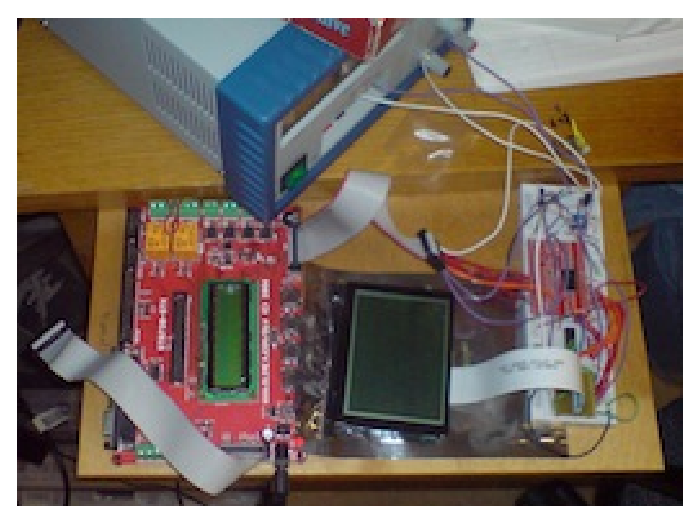
\includegraphics[width=2.5in,keepaspectratio]{results/figures/lcd_bench_test.eps}
}
\subfigure[CAN Bench test]{
  \label{fig:can_bench_test}
  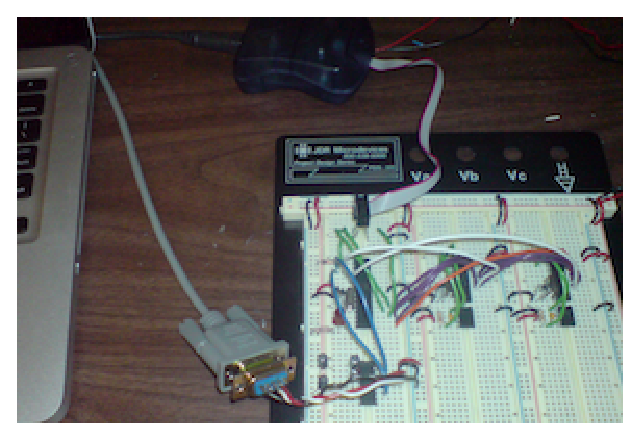
\includegraphics[width=2.5in,keepaspectratio]{results/figures/can_bench_test.eps}
}
\caption{Photographs of the driver control module bench-test experiments.}
\label{fig:bench_experiments}
\end{figure}

\subsection{Graphics Display}

Once all the hardware bugs with the driver interface module had been corrected, it was possible to continue writing the LCD interfacing software that had been started during the initial LCD testing. The external memory interface circuitry described in Sec.\ \ref{sec:lcd_module_data_interface} worked without issue. Figure \ref{fig:driver_interface_lcd} shows the LCD displaying a sample bitmap from the manufacturer.

\begin{figure}[H]
 \centering
 \includegraphics[width=5in,keepaspectratio]{results/figures/driver_interface_lcd.eps}
 \caption{Photograph of the LCD under test.}
 \label{fig:driver_interface_lcd}
\end{figure}

\subsection{Vehicle Dynamic Adjustment}

A menu system for adjusting the vehicle dynamic parameters was implemented. Turning the \emph{param} knob on the driver interface module scrolls through the list of parameters. Figure \ref{fig:driver_interface_menu} shows the LCD module displaying the parameter menu. Also visible is the system time, drawn at the top centre, the telemetry module signal strength indicator in the top right. All text in Fig. \ref{fig:driver_interface_menu} is drawn using the custom 16x16 font described in Sec.\ \ref{sec:lcd_module_font_loading}.

\begin{figure}[h!]
 \centering
 \includegraphics[width=3in,keepaspectratio]{results/figures/driver_interface_menu.eps}
 \caption{Photograph of the driver interface module displaying the parameter menu.}
 \label{fig:driver_interface_menu}
\end{figure}
